% Don't type any content in this file. Put all the text in the chapters folder
% for modularity.

% setting the graphics path to get images
\graphicspath{ {chapters/images/} }
% command for blank page
\newcommand{\blankpage}{
\newpage
\thispagestyle{plain}
\mbox{}
\newpage
}
% add a box around text in images and also textwrap
\lstset{
    frame=single,
    breaklines=true,
    postbreak=\raisebox{0ex}[0ex][0ex]{\ensuremath{\color{black}\hookrightarrow\space}}
}
% command for paragraph with a line before it
\newcommand{\para}{
\medskip
\par
}
% Quote the author
\def\signed #1{{\leavevmode\unskip\nobreak\hfil\penalty50\hskip2em
  \hbox{}\nobreak\hfil(#1)%
  \parfillskip=0pt \finalhyphendemerits=0 \endgraf}}

\newsavebox\mybox
\newenvironment{aquote}[1]
  {\savebox\mybox{#1}\begin{quote}}
  {\signed{\usebox\mybox}\end{quote}}

%make sure RepOk is never broken
\hyphenation{RepOk}

% adding chapters from their respective tex files
\chapter{Introduction}
Testing plays a vital role in developing reliable systems. However, testing manually is expensive and tedious. Researchers have long recognized the benefits of using specifications in automated testing~\cite{...}. While the initial use of specifications was largely in academic settings, the last fifteen years have seen much progress in developing tools that can make use of specifications to test real applications, e.g., by generating test inputs automatically using constraint solving \cite{demilli1991constraint,gotlieb1998automatic,howden1977symbolic,huang1975approach,king1976symbolic,korel1996automated,legeard2002automated,marinov2001testera}.

\medskip
\para
The focus of our work is test input generation using imperative predicates, which was introduced by the \emph{Korat} approach \cite{boyapati2002korat}. Korat takes a given Java method, called \emph{repOk}, that returns a \emph{boolean} method, and systematically explores the input space of the predicate to enumerate inputs for which \emph{repOk} returns \emph{true}. The focus of Korat’s generation is structurally complex data, e.g., recursive data structures allocated on the program heap. The input spaces to explore for such recursive structures are often huge.  Korat performs a bounded exploration defined by a \emph{finitization} given by the user to bound the input size. Korat efficiently prunes the space of candidate inputs for the \emph{repOk} method by executing it on candidate inputs and monitoring the object fields that \emph{repOk} accesses in deciding if the properties are satisfied. Moreover, Korat prunes from search candidates that are isomorphic to any candidate already evaluated, thereby further reducing the number of candidates to consider by a considerable factor.

\para
While Korat generates inputs effectively, its correctness and efficiency rely on two assumptions about the \emph{repOk} methods.  For correctness, Korat assumes the \emph{repOk} methods do not use the Java reflection API for field accesses; the use of reflection renders Korat unable to enumerate all desired inputs.  For efficiency, Korat assumes the \emph{repOk} methods are written such that they only access fields that are necessary to check the properties; the use of unnecessary field accesses by \emph{repOk} renders Korat's pruning ineffective.

\para
In this thesis, we address both these limitations.  To support reflection, we build on the core Korat to enhance it such that it can monitor field accesses based on reflection.  To deal with unnecessary field accesses, we present a tool called \emph{RepOkValidator} that points out these field accesses so that the user can choose to fix them to makes sure Korat’s efficiency remains unaffected. 


\section{Korat : A solver for imperative predicates}
A \emph{constraint} is a formula that specifies some property of a set of variables. For example, the constraint \emph{x \textgreater 0 \&\& x \textless 10}, specifies that the value of \emph{x} needs to be between zero and ten. Constraint solving amounts to finding solutions to constraints, i.e assignments to variables that make the constraint formula true. For example, \emph{x = 5} is a solution for the above constraint formula. The main idea is to represent the property of the desired test inputs as a constraint such that the solution to the constraint translates to a test input. Though there have been other approaches that focussed on constraints where variables are integers or arrays of integers \cite{demilli1991constraint,huang1975approach,king1976symbolic,korel1996automated}. Korat \cite{boyapati2002korat} is the first tool that solved constraints for structurally complex inputs.

\para
Korat understands constraints as imperative predicates written by the user. An \emph{imperative predicate} is a piece of code that takes an input structure and determines its validity. Solving an imperative predicate amounts to finding structures for which the predicate returns \emph{true}; Korat calls these structures valid structures. Imperative predicates give the user an operational way of expressing declarative constraints that identify the desired test inputs. The user provides an imperative predicate, written in Java, that returns true if the input structure satisfies the required property and \emph{false} otherwise. Every valid structure translates into a test input.

\para
Korat takes as an input; a java \emph{predicate} and a \emph{finitization} that bounds the size of the input structures and produces all valid \emph{nonisomorphic} structures within the given bounds as an output. A finitization specifies bounds for the number of objects in a structure and the possible values for the fields of these objects. Korat generates all valid structures by systematically searching the structure space defined by the finitization. Korat prunes the search space by monitoring the execution of the predicate and determining the fields of the structure accessed by the predicate before it returns the result. The efficiency of the pruning depends not only on the set of valid structures (usually very small compared to the size of the structure space) but also on the way the imperative predicate is written. An ill-written predicate might always read all the fields of a structure before returning the result, thereby forcing Korat to explore almost the entire structure space. In chapter 2, we will see an example of this behavior.


\section{Reflection and its importance}
\noindent Formally, reflection can be split into three main aspects \cite{bracha2004mirrors,mostinckx2009mirror}:
\begin{itemize}
\item \emph{Introspection}: the ability of a program to examine itself.
\item \emph{Self-modification}: the ability of a program to alter its structure.
\item \emph{Intercession}: the ability of a program to alter its behaviour.
\end{itemize}

\para
Unfettered run-time modification of a system is dangerous, since it can have subtle, unintended consequences. However careful use of reflection allows programmers to bend a language to their particular circumstances rather than the other way round. Most dynamically typed languages are capable of introspection; many are capable of self-modification; relatively few are capable of intercession. Korat is primarily written in Java which is a statically typed language that only supports the introspective \cite{maes1987concepts} aspects of reflection.Java Reflection makes it possible to inspect classes, interfaces, fields and methods at runtime, without knowing the names of the classes, methods etc. at compile time. It is also possible to instantiate new objects, invoke methods and \emph{get/set} field values using reflection.

\para
Korat monitors the field accesses made by the imperative predicate written by the user and prunes the search space accordingly. Since java supports field access using reflection, it is important to make sure that Korat also monitors field accesses using reflection. This property will become more useful when Korat is implemented in a dynamically typed language like ruby/python. 

\section{Static Analysis}
Static program analysis is the analysis of a piece of code without actually executing the piece of code. The sophistication of the analysis performed by different tools varies from those that only consider the behavior of individual statements and declarations, to those that include the complete source code of a program in their analysis. Since a badly written predicate can deteriorate the efficiency of Korat, a static analysis of the predicate can point out places (if any) where the predicate can be improved. Chapter 4 presents \emph{RepOkValidator}, a tool that  uses \emph{def-use} analysis to check if the predicate written by the user affects the efficiency of Korat.

\para
A def-use analysis is a data-flow analysis which helps in statically accumulating def-use and use-def chains. A use-definition chain is a data structure that consists of a use, U, of a variable, and all the definitions, D, of that variable that can reach that use without any other intervening definitions. Once the RepOkValidator has access to the use-def chain of the predicate, it checks the chain to see if a few properties (mentioned in chapter 4) that affect Korat’s efficiency are not violated.

\section{Organization}
The remainder of this thesis is organized as follows. Chapter 2 illustrates with examples, scenarios where Korat underperforms. Chapter 3 talks about adding reflection to Korat. Chapter 4 presents a static analysis tool that can be used to validate a predicate written by the user. Chapter 5 presents a small library that can be used for code reuse in predicates. Chapter 6 compares usage of predicates that use reflection and a predicate that does not use reflection, with Korat and shows how Korat performs when reflection is not supported. Chapter 7 discusses other approaches that people have used to improve Korat and also suggests some future work.

\chapter{Shortcomings of Korat}
This chapter presents two scenarios where Korat\cite{boyapati2002korat} fails to generate the \emph{best} possible results it is capable of producing with its algorithm. The first example shows how Korat malfunctions by terminating before exploring all the states when reflection is used in the predicate written by the programmer. The second example shows how korat explores more states than required when the predicate written by the programmer doesn’t return the result as soon as possible. Both examples use a binary tree data structure to illustrate a predicate method that validates a linked data structure. The shortcomings observed in both the examples will also apply for an array-based data structure, like a heap.

\section{Usage of reflection for field access}
In this example, we use two different ways of field access using reflection to illustrate both the ways a programmer can use reflection to access a field. Figure \ref{fig:btreeDirectRepOk} shows the java code for a binary tree implementation. Each object of the class \emph{BinaryTree} represents a binary tree. The value of the \emph{size} field is the number of nodes in the tree. Objects in the inner class \emph{Node} represent nodes of the tree. To use Korat, the programmer needs to provide an imperative predicate that checks the validity of inputs. It is called \emph{repOk} and it typically checks the representation invariant or class invariant of the corresponding data structure. \\


\begin{figure}
\centering
\begin{lstlisting}[language=Java]
class BinaryTree {
    Node root;    // root node
    int size;    // number of nodes in the tree
    static class Node {
        Node left;    // left child
        Node right;    // right child
    }

    boolean repOK() {
        // checks that empty tree has size zero.
        if (root == null) return size == 0;
        Set visited = new HashSet();
        visited.add(root);
        LinkedList workList = new LinkedList();
        workList.add(root);
        // loop checks that the object graph is a tree.
        while (!workList.isEmpty()) {
            Node current = (Node) workList.removeFirst();
            if (current.left != null) {
                if (!visited.add(current.left))
                    return false;
                workList.add(current.left);
            }
            if (current.right != null) {
                if (!visited.add(current.right))
                    return false;
                workList.add(current.right);
            }
        }
        // checks that the size is consistent.
        return (visited.size() == size);
    }
}
\end{lstlisting}
\caption{Binary tree example with repOk using direct field access.}
\label{fig:btreeDirectRepOk}
\end{figure}

\para
Figure \ref{fig:btreeDirectRepOk} also shows the \emph{repOk} method that uses direct field access for \emph{BinaryTree}; \emph{repOk} is a predicate that checks the input is indeed a valid binary tree with the correct size. First, \emph{repOk} checks if the tree is empty. If not, \emph{repOk} checks that there are no undirected cycles in the object graph reachable from the \emph{root} field along the \emph{left} and \emph{right} fields. It finally checks that the number of nodes reachable from the root is the same as the value of field \emph{size}. The programmer can use Korat to generate valid test inputs for any method that requires a \emph{BinaryTree} instance as an input. Each binary tree generated will satisfy the \emph{repOk}. To limit the number of inputs, the programmer provides Korat with a finitization that specifies bounds on the number of objects in the data structures and on the values in the fields of these objects. For trees, the finitization specifies the maximum number of nodes and the possible elements. A tree is considered to be in scope n, if it has at most n nodes and n elements. We can use integers from \emph{1 to n} for the \emph{size} field inside the \emph{BinaryTree} class.

\para
Given a finitization and a value for scope, Korat generates all non-isomorphic structures that can be formed for a given data structure. In our example, two binary trees are isomorphic if they have the same underlying graph and the elements, irrespective of the identity of the actual nodes in the trees. 

\begin{figure}
\centering
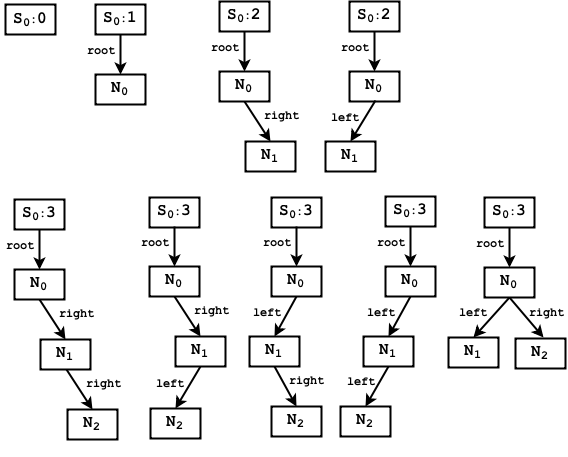
\includegraphics[width=12cm,height=8cm,keepaspectratio]{korat_instances_binary_tree_size_3}
\caption{Binary trees that Korat generates for scope three.}
\label{fig:btreeKoratGenScopeThree}
\end{figure}

\para
When using the \emph{repOk} shown in Figure \ref{fig:btreeDirectRepOk} with a scope of three, Korat generates 90 non-isomorphic candidate structures of which 9 structures end up being valid as they pass the \emph{repOk}. Figure \ref{fig:btreeKoratGenScopeThree} shows the trees that Korat generates for scope three. Each tree consists of one \emph{BinaryTree} object S0 and upto three \emph{Node} objects (N0, N1, N2). For each object, the value and the identity of primitive fields and \emph{Node} objects is shown. Edges represent the values of reference fields with no edge for \emph{null}.

\para
To enable efficient search for valid structures, Korat encodes each structure with a state, and each finitization bounds the state space. Korat uses backtracking to systematically search this state space to find all valid structures. Based on a finitization for the input structures of the predicate, Korat first initializes the state space of structures. Korat then builds candidate structures and executes the predicate on them to check their validity. Korat monitors these executions to dynamically determine which parts of the candidate the result of the predicate depends on. More specifically, Korat monitors the fields of the candidates the execution accesses. If the predicate returns \emph{true}, Korat outputs the candidate as a valid structure for testing. Otherwise, if the predicate returns false or an exception is thrown in the middle of execution, Korat skips the candidate. Korat then backtracks on the values of the accessed fields, to generate the next candidate. Finally, Korat terminates when it explores the entire search space. 

\begin{figure}
\centering
\begin{lstlisting}[language=Java]
boolean repOK() {
    // checks that empty tree has size zero.
    if (root == null) return size == 0;
    Set visited = new HashSet();
    visited.add(root);
    LinkedList workList = new LinkedList();
    workList.add(root);
    // loop checks that the object graph is a tree.
    while (!workList.isEmpty()) {
        Node current = (Node) workList.removeFirst();
        if ((Node)BinaryTree.class.getDeclaredField(``left'').get(current) != null) {
            if (!visited.add(current.left)) 
                return false;
            workList.add(current.left);
        }
        if (current.right != null) {
            if (!visited.add(current.right))
                return false;
            workList.add(current.right);
        }
    }
    // checks that the size is consistent.
    return (visited.size() == size);
}
\end{lstlisting}
\caption{RepOk using the java reflection API for accessing the left child of a Node inside the loop.}
\label{fig:btTreeReflectionRepOK}
\end{figure}

\para
Korat monitors field accesses by replacing direct field accesses with accessor methods that make note of the access and hence affect the way Korat generates candidates. Figure \ref{fig:btTreeReflectionRepOK} and figure \ref{fig:btTreeUserReflectionRepOK} show repOKs that use reflection to access fields in the \emph{BinaryTree} class.

\begin{figure}
\centering
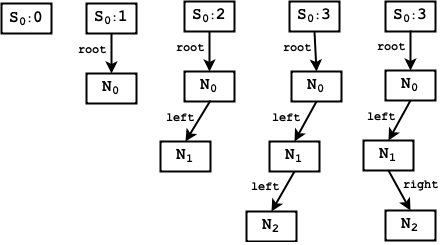
\includegraphics[width=11cm,height=6cm,keepaspectratio]{korat_instances_reflection_binary_tree_size_3}
\caption{ Binary trees that Korat generates for scope three when repOk uses reflection.}
\label{fig:btreeReflectKoratGenScopeThree}
\end{figure}

\para
The main difference between the \emph{repOk} that uses direct access (shown in figure \ref{fig:btreeDirectRepOk}) and the \emph{repOk} that uses the java reflection API (shown in figure \ref{fig:btTreeReflectionRepOK}) is the access of just one field.The latter \emph{repOk} accesses the \emph{left} child of every \emph{Node} object using the java reflection API instead of direct field access. Since Korat is capable of monitoring only direct field accesses, it doesn’t account for this field access. This ends up affecting the generation of candidates and produces fewer trees than the direct access \emph{repOK}, for the same scope. Figure \ref{fig:btreeReflectKoratGenScopeThree} shows the binary tree structures generated when the repOk in figure \ref{fig:btTreeReflectionRepOK} is used to validate the binary tree candidates that Korat explores. Korat generates only 28 non-isomorphic candidate structures of which 5 structures end up being valid as they pass the repOk.

\begin{figure}
\centering
\begin{lstlisting}[language=Java]
boolean repOK() {
    // checks that empty tree has size zero.
    if (root == null) return size == 0;
    Set visited = new HashSet();
    visited.add(root);
    LinkedList workList = new LinkedList();
    workList.add(root);
    // loop checks that the object graph is a tree.
    while (!workList.isEmpty()) {
        Node current = (Node) workList.removeFirst();
        if ((Node)ReflectionUtils.getFieldValue(current, ``left'') != null) {
            if (!visited.add(current.left))
                return false;
            workList.add(current.left);
        }
        if (current.right != null) {
            if (!visited.add(current.right))
                return false;
            workList.add(current.right);
        }
    }
    // checks that the size is consistent.
    return (visited.size() == size);
}
\end{lstlisting}
\caption{RepOk using the user written reflection API for accessing the left child of a Node inside the loop.}
\label{fig:btTreeUserReflectionRepOK}
\end{figure}

\para
This proves that Korat’s algorithm is drastically affected even if a single field access is done using reflection. To make sure Korat functions as expected and continues to remain complete, it is essential to account for field accesses that use reflection, including direct field accesses. Figure \ref{fig:btTreeUserReflectionRepOK} shows another version of \emph{repOk} that uses a user written method to access the \emph{left} field of every \emph{Node} object. It is assumed that this method uses java reflection API within the method body. Using this version of \emph{repOk} to generate binary tree inputs also produces the same trees shown in figure \ref{fig:btreeReflectKoratGenScopeThree} as Korat is capable of monitoring only direct field accesses. 


\section{Inefficient predicates}
Korat claims to efficiently generate all valid non-isomorphic structures even for large state spaces. The search pruning that Korat performs allows Korat to explore only a tiny part of the state space. The ratio of the number of candidate structures considered and the size of the state space shows that the key to effective pruning is backtracking based on fields accessed during predicate execution. Korat usually performs extremely well when the user written predicate returns a \emph{true/false} as soon as it knows the result. Figure \ref{fig:btreeDirectRepOk} shows a \emph{repOk} of a \emph{BinaryTree} that checks for three violations that can render a candidate as an invalid binary tree. The \emph{repOk} returns \emph{false} as soon as it knows that the candidate has violated one of the three rules for a graph to be a binary tree.

\begin{figure}
\centering
\begin{lstlisting}[language=Java]
boolean repOK() {
    boolean result = true;
    // checks that empty tree has size zero.
    if (root == null) result = (size == 0);
    Set visited = new HashSet();
    LinkedList workList = new LinkedList();
    if (root != null) {
        visited.add(root);
        workList.add(root);
    }
    // loop checks that the object graph is a tree.
    while (!workList.isEmpty()) {
        Node current = (Node) workList.removeFirst();
        if (current.left != null) {
            if (!visited.add(current.left))
                result = false;
            else workList.add(current.left);
        }
        if (current.right != null) {
            if (!visited.add(current.right)) 
                result = false;
            else workList.add(current.right);
        }
    }
    // checks that the size is consistent.
    if(!result) result = (visited.size() == size);
    return result;
}
\end{lstlisting}
\caption{RepOk that doesn’t return the result as soon as it knows it.}
\label{fig:bTreeInefficient}
\end{figure}

\para
When using the \emph{repOk} shown in Figure \ref{fig:btreeDirectRepOk} with a scope of three, Korat generates 90 non-isomorphic candidate structures of which 9 structures end up being valid. The \emph{repOk} shown in figure \ref{fig:bTreeInefficient} has the exact same functionality and also generates the same valid structures as the \emph{repOk} in figure \ref{fig:btreeDirectRepOk} but, it ends up generating 893 candidate structures for scope three which is an order of magnitude more than the number of candidate structures generated by the \emph{repOk} in figure \ref{fig:btreeDirectRepOk}. For a larger scope, we can observe an increase by multiple orders of magnitude. The \emph{repOk} in figure \ref{fig:bTreeInefficient} ends up being an inefficient predicate for generation as it does not return \emph{true/false} right after it knows the result. This is one of the reasons why Korat doesn’t make any promises about its efficiency as it is partly dependant on the predicate written by the user. Though this is not a shortcoming of Korat, it is one of the situations where the effectiveness of Korat is nullified.

\chapter{Adding reflection to Korat}
In this chapter, we will look at the reflection support added in the improvised Korat. In section 2.1 of chapter 2, we observed that using reflection for field accesses inside the predicate written by the user will make korat terminate its search before it finishes exploring all the states. This is because, the field accesses are not accounted for and Korat’s search algorithm primarily depends on monitoring field accesses.

\section{Instrumentation of field accesses}
Korat monitors direct field accesses by instrumenting the code written by the user. Korat performs source-source translation that instruments all classes whose objects appear in finitizations. Korat uses the observer pattern ~/cite{...} to monitor executions of the predicate (and transitively invoked methods) to build a stack of accessed fields. For each class, the instrumentation adds a special constructor and a field for the observer, as shown in figure 3-1. For each field in a class, the instrumentation adds an identifier field and getter/setter methods for the field. Finally, in the code for repOk and all the methods that repOk transitively invokes, the instrumentation replaces each read/write of the field with the generated getter/setter methods respectively.

\par
The special constructor generated by the instrumentation initializes the korat\_observer field and the identifiers for all fields. The finitization uses the special constructor to initialize all objects with an observer and to initialize each identifier field to a unique integer. Other than the identifier, each field has a korat\_get and a korat\_set method method. During the execution of these methods, they first notify the observer that the field is being accessed and then actually return the field or set the value for the field based on the setter/getter invoked.


\begin{figure}
\centering
\begin{lstlisting}[language=Java]
class BinaryTree {
    korat.Observer korat_observer;  // observer for this object
    // special constructor to initialize the observer and field ids
    BinaryTree( korat.Observer observer, korat.Ids id) {
        korat_observer = observer;
        korat_id_root = id.getNextId();
        korat_id_size = id.getNextId();
    }
    Node root; // root node
    int korat_id_root; //identifier for root node
    //special get method for the root field
    Node korat_get_root(){
        korat_observer.notify_get(korat_id_root);
        return root;
    }
    //special set method for the root field
    void korat_set_root(Node value){
        korat_observer.notify_set(korat_id_root);
        root = value;
    }
    int size; // number of nodes in the tree
    int korat_id_size; //identifier for size field
    //special get method for the size field
    int korat_get_size(){ 
        korat_observer.notify_get(korat_id_size);
        return size;
    }
    //special set method for the size field
    void korat_set_size(int value){ 
        korat_observer.notify_set(korat_id_size);
        size = value;
    }
   
    // a repOk where all the field accesses are 
    // replaced with the korat getter and setter methods.
}
\end{lstlisting}
\caption{Instrumentation of BinaryTree class by Korat.}
\label{fig:btTreeInstrumentationKorat}
\end{figure}


\section{Adding reflection to Instrumentation}
Korat fails to monitor field accesses that use reflection. In order to make sure field accesses that use reflection are monitored by Korat, the instrumentation needs to make sure it accounts for reflection. Figure 3-2 shows all the methods in the java.reflect.Field class that can used to access a field using the java reflection API. The figure does not show methods that can be used to set the value of field using reflection but, it should be straightforward to find the counterparts of the getter methods from the documentation. The Korat instrumentation needs to look for invocation of these methods in the predicate written by the user and replace them with the getFieldValue method from the ReflectionUtils class as shown in figure 3-2. We haven’t modified the implementation of Korat instrumentation to account for reflection based field access. All experiments were done by manually using the getFieldValue method in place of the methods from the Field class.

\begin{figure}
\centering
\begin{lstlisting}[language=Java]
Object ReflectionUtils.getFieldValue(Object obj, String fieldName)

Object get(Object obj)
boolean getBoolean(Object obj)
byte getByte(Object obj)
char getChar(Object obj)
double getDouble(Object obj)
float getFloat(Object obj)
int getInt(Object obj)
long getLong(Object obj)
short getShort(Object obj)

\end{lstlisting}
\caption{Methods of the field class that the instrumentation needs to replace with the getFieldValue method.}
\label{fig:fieldClassInstrumentationMethods}
\end{figure}

\section{Unaccounted field accesses}
Korat monitors direct field accesses by instrumenting the code written by the user. Korat’ search algorithm is primarily dependant on field accesses and extra field accesses might lead to the decrease of efficiency of Korat, as shown in section 2.2. There can be situations where the programmer doesn’t want to use the field access to determine the result of the predicate. For example, the user just wants to log the current value of the field, or send to an external observer. Since Korat monitors every field access by instrumenting the repOk written by the user, we have provided an indirect way to get/set the value of a field without accounting for the access.

\par
The public static method unaccountedAccess in the ReflectionUtils class offers a way to access an object without accounting for its access. Since Korat already doesn’t account for reflection, we don’t have to worry about the existing instrumentation of Korat, instrumenting this method call. Figure 3-3 shows an example usage of the method for logging. It is important to note that the static analysis tool that we developed (RepOkValidator from chapter 4) also, doesn’t consider this as an access and hence doesn’t raise any violations when this method is used to access a field.


\begin{figure}
\centering
\begin{lstlisting}[language=Java]
boolean repOK() {
    // checks that empty tree has size zero.
    if (root == null) return size == 0;
    Set visited = new HashSet();
    visited.add(root);
    LinkedList workList = new LinkedList();
    workList.add(root);
    // loop checks that the object graph is a tree.
    while (!workList.isEmpty()) {
        Node current = (Node) workList.removeFirst();
        if (current.left != null) {
            if (!visited.add(current.left)) return false;
            workList.add(current.left);
        }
        if (current.right != null) {
            if (!visited.add(current.right)) return false;
            workList.add(current.right);
        }
    }
    // Korat’s search is not affected by the following access.
    if(visited.size() != (int)ReflectionUtils
             .unaccountedAccess(this,”size”)){
        System.out.println(“Size mismatch, need to change size”);
    }
    // checks that the size is consistent.
    return (visited.size() == size);
}
\end{lstlisting}
\caption{BinaryTree repOk using unaccounted field access for logging.}
\label{fig:bTreeUnaccountedFieldAccess}
\end{figure}

\chapter{Static analysis to check predicate}
\label{ch:static-analysis}
This chapter presents a static analysis tool (we call it the RepOkValidator) to check the predicate written by the user to use with Korat. A predicate is a piece of code that takes an input (a candidate structure in our case) and returns a boolean that represents, if the predicate has a proper representation. Our tool will statically analyze the predicate written by the user and point out places where it can be changed to optimize the execution of Korat when the predicate is used with Korat.

\section{Conditions}
\label{sec:static-analysis-conditions}
As we have seen in chapter \ref{ch:shortcomings-of-korat}, the execution of Korat is partly dependant on the predicate written by the user. A repOk that doesn’t return the result as soon as possible, will end up heavily affecting the pruning mechanism of Korat. Korat requires\cite{marinov2005automatic} that the following conditions hold good for a user written predicate - 

\begin{aquote}{Darko Marinov}
C1 : Each execution of the predicate terminates, and either returns a true or a false.\\
C2 : No execution of the predicate depends on the actual allocation address of the candidate object or its fields.(This holds for java predicates if no execution invokes \emph{System.identityHashCode} method.)\\
C3 : Each field that the predicate accesses is either a part of the candidate structure or a field of some object that the predicate locally allocates. In other words, the execution does not access global data through static fields.\\
\end{aquote}

\para
It is possible to make a guarantee about the Korat’s efficiency (the number of candidates considered by Korat) if the user written predicate follows the conditions below, in addition to the conditions specified by Korat. In other words, the following conditions only affect the efficiency of Korat, unlike C1-C3 which affect the correctness of the output generated by Korat. The following conditions assume that a fixed amount of space (variable length data structures like boolean arrays/lists are not used) is allocated for the booleans used by the predicate. 
\begin{itemize}
\item C4 : If the return value of the predicate is a variable then, it is set at most once between the time of its declaration and its return along any path of execution.
\item C5 : If the return value is a conjunction or a disjunction of multiple boolean variables then, each variable is set at most once during the time between its declaration and usage in deciding the return value.
\item C6 : No fields are accessed (chapter \ref{ch:adding-reflection} describes a way to access the fields without Korat accounting for the access) between the time of setting the return value and the actual return of the value.
\end{itemize}

\para
The above conditions were derived from observing the results of executions of Korat with various predicates that resulted in the same valid structures but considered different number of candidate structures.

\section{Choosing static analysis over dynamic analysis}
\label{sec:choosing-static-over-dynamic}
Given a predicate, it is possible to use a static or dynamic analysis of the predicate to derive detailed information about the predicate. The user of Korat needs to write a predicate so that conditions C1-C3 hold so that Korat works correctly. The user also can optionally make sure that C4-C6 hold to ensure that Korat takes the least amount of time possible to execute. 

\para
Dynamic analysis is the testing and evaluation of a piece of code during runtime. Dynamic analysis reveals subtle faults whose cause is often complex to be discovered by static analysis. It is usually more time consuming than a static analysis. Static analysis is the testing and evaluation of a piece of code by examining it, without executing it. It examines all possible execution paths and variable values, not just those invoked during execution. The only condition that can’t be checked is C1, as it is the halting problem. Since every other condition can be checked using a static analysis, we decided to use static analysis over dynamic analysis in the interest of avoiding the execution time overhead of dynamic analysis.

\section{RepOkValidator}
\label{sec:repokvalidator}
The RepOkValidator is a static analysis tool that will analyze the predicate written by the user. It will print all the violations in the form of a log. The log can help the user to ensure that the predicate will execute in the least amount of time possible, when used with Korat. In other words, the RepOkValidator will print violations of conditions C2-C6 and localize them in the predicate to make it easier for the user to fix the violations. It is important to understand that violations of type C2 and C3 need to be fixed before using the predicate with Korat. Korat requires that condition C1-C3 hold good for it work properly. On the other hand, It is optional for the user to fix violations of type C4-C6 as they just affect the efficiency of Korat as opposed to the correctness. As of today, the RepOkValidator is a standalone tool that can optionally be used by the user to validate the predicate written before using it with Korat.

\para
For each condition to hold good, the RepOkValidator needs to look for specific violations of the conditions in the predicate. 
\begin{itemize}
\item C2 : will be violated if the predicate written by the user invokes the System.identityHashCode method.
\item C3 : will be violated if any fields accessed in the predicate don’t belong to the candidate class or the fields accessed are static.
\item C4 : will be violated if the return value is assigned a value more than once, from the time it is defined to the time it is returned, in any path of execution.
\item C5 : will be violated if any of the variables that make up the result are assigned a value more than once from the time they are defined to the time they are returned, in any path of execution.
\item C6 : will be violated if any of the candidate class fields are accessed once all of the fields that make up the return value are assigned a value.
\end{itemize}

\para
To be able to detect the violations, we build def-use chains and use-def chains of all variables in the predicate. We also collect data about all method invocations, including the parameters used to invoke the methods. Once we have this data, RepOkValidator traverses the use-def and def-use chains to detect violations and logs them for user reference.

\section{Implementation}
\label{sec:implementation}
The implementation of RepOkValidator uses Soot ~/cite{..}, a java bytecode optimization framework. The framework is implemented in Java and support three intermediate representations of java bytecode. RepOkValidator uses the intermediate representation called Jimple as it is an ideal representation for static analysis. Jimple is a 3-address code representation of bytecode, which is typed and does not include the 3 address code equivalent of a jsr (jump to subroutine) instructions.

\para
The RepOkValidator takes the data structure that needs to be analyzed as a command line argument and passes the argument on to Soot, for it convert the class into jimple. Once the code is converted to jimple, the RepOkValidator looks for all the methods that return a boolean and have a method name that starts with repOk and take no arguments. For each such method, the RepOkValidator does intraprocedural analysis to extract the def-use and use-def chains of all variables in the method. After extracting the def-use and use-def chains, RepOkValidator sequentially validates the predicate for each condition in C2-C6 and adds violations to the violation log for user’s reference.

\para
Finally, if the violation log is empty, the RepOkValidator prints that the predicate passed the test. This means that the predicate will work with Korat and will also help Korat perform efficiently.

\section{Example}
\label{sec:static-analysis-example}
In this section, we will be looking at two predicates written for a BinaryTree shown in figure \ref{fig:btreeDirectRepOk}. The first example will show a faulty predicate that will not work with Korat as it doesn’t obey conditions C2 and C3. The second example will show an inefficient predicate which will work with Korat but can be optimized using the log messages produced by the RepOkValidator.

\subsection{Faulty Predicate}
\label{sec:faulty-predicate}
Figure \ref{fig:repOkKoratSatisfyCorrectness} shows a repOk that a user can write to generate non-isomorphic BinaryTree structures. The repOk won't reliably work with Korat as it violates the conditions that need to be fulfilled for Korat to function properly. To be specific, the repOk violates condition C3 from section \ref{sec:static-analysis-conditions}. It violates C3 by using the MAX\_SCOPE\_PARAM field from the Settings class (shown in figure \ref{fig:repOkKoratSatisfyCorrectness}).The field can be changed during the Korat search and hence will make the Korat search return wrong/incomplete results, if changed to a different value.

\begin{figure}
\centering
\begin{lstlisting}[language=Java]
public class Settings {
    public static int MAX_SCOPE_PARAM = 3;
}

boolean repOKFaulty() {
    //makes sure the size is not more than limit
    if (size > Settings.MAX_SCOPE_PARAM) 
        return false;
    // checks that empty tree has size zero.
    if (root == null) return size == 0;
    Set visited = new HashSet();
    visited.add(root);
    LinkedList workList = new LinkedList();
    workList.add(root);
    // loop checks that the object graph is a tree.
    while (!workList.isEmpty()) {
        Node current = (Node) workList.removeFirst();
        if (current.left != null) {
            if (!visited.add(current.left))
                return false;
            workList.add(current.left);
        }
        if (current.right != null) {
            if (!visited.add(current.right))
                return false;
            workList.add(current.right);
        }
    }
    // checks that the size is consistent.
    return (visited.size() == size);
}

\end{lstlisting}
\caption{RepOk that doesn’t work with Korat as it doesn’t satisfy condition C3.}
\label{fig:repOkKoratSatisfyCorrectness}
\end{figure}

\para
When the predicate is analyzed using the RepOkValidator, it prints a log of the violations that need to be fixed by the user to make sure Korat functions properly when the repOk is used with Korat. Figure \ref{fig:repOkKoratSatisfyCorrectnessLog} shows the logs printed by the RepOkValidator. Each log will mention the kind of the violation, the line number at which the violation is made, the predicate method inside which the violation is made and the class to which the repOk belongs to. Since all the violations shown by figure \ref{fig:repOkKoratSatisfyCorrectnessLog} belong to C1-C3, it is important that the user fixes all the violations to ensure that Korat will function properly with the predicate.

\begin{figure}
\centering
\begin{lstlisting}[language=Java]
-------------- Analyzing repOkFaulty from edu.utexas.BinaryTree ------------
Condition C3 violated : usage of a static field - MAX_SCOPE_PARAM from class edu.utexas.BinaryTree$Settings at line 54 inside repOKEfficient in edu.utexas.BinaryTree
------------ repOkFaulty did not pass the test ------------
\end{lstlisting}
\caption{Violation log generated by the RepOkValidator when the faulty repOk is analyzed.}
\label{fig:repOkKoratSatisfyCorrectnessLog}
\end{figure}

\subsection{Inefficient Predicate}
\label{sec:inefficient-predicate}
Figure \ref{fig:repOkMultipleBooleanVariables} shows another repOk that the programmer can write to generate non-isomorphic BinaryTree structures. This time the repOk works with Korat as it does not violate conditions C1-C3. Even though the repOk generated all valid non-isomorphic structures when used with Korat, it considered way too many candidate structures to generate them. This is because the predicate violates conditions C5 and C6. Since violating conditions C4-C6 affects the efficiency of Korat, it is observed that the execution of Korat with this predicate takes more time compared to the predicate in figure \ref{fig:btreeDirectRepOk}, which passes the RepOkValidator test.

\para
The repOk violates C5 because the boolean variable acyclic is defined twice before it is returned. Since the result of the predicate depends on the variable, it is possible to return the result right after setting the value of acyclic for the first time. It also violated C6 as there are multiple field references after setting the value of the variable acyclic and before it is actually returned as a result for the predicate.

\begin{figure}
\centering
\begin{lstlisting}[language=Java]
boolean repOKMultipleVariables() {
    boolean sizeOk = true, acyclic = true;
    // checks that empty tree has size zero.
    if (root == null) sizeOk = (size == 0);
    Set visited = new HashSet();
    visited.add(root);
    LinkedList workList = new LinkedList();
    workList.add(root);
    // loop checks that the object graph is a tree.
    while (!workList.isEmpty()) {
        Node current = (Node) workList.removeFirst();
        if (current.left != null) {
            if (!visited.add(current.left)) acyclic = false;
            else workList.add(current.left);
        }
        if (current.right != null) {
            if (!visited.add(current.right)) acyclic = false;
            else workList.add(current.right);
        }
    }
    // checks that the size is consistent.
    return acyclic && sizeOk && (visited.size() == size);  
}
\end{lstlisting}
\caption{RepOk that uses multiple boolean variables to decide its result. It violates C5 and C6 and ends up affecting the efficiency of Korat.}
\label{fig:repOkMultipleBooleanVariables}
\end{figure}

\para
It is also worth noticing that multiple boolean variables go into deciding the result of the predicate. This is very common for complex, recursive data structures like the BinaryTree. In situations like this, the RepOkValidator proves to be extremely useful as it exactly points out the places at which the violations are made. Once the programmer knows the places at which the violations are made, it should be straightforward to fix the predicate to ensure maximum efficiency. Figure \ref{fig:repOkKoratSatisfyEfficiencyLog} shows the violation log that gets generated when the repOk shown in figure \ref{fig:repOkMultipleBooleanVariables} is analyzed with the RepOkValidator.

\begin{figure}
\centering
\begin{lstlisting}[language=Java]
-------------- Analyzing repOKMultipleVariables from edu.utexas.BinaryTree ------------
Condition C5 violated : redefinition of field acyclic at line 91 inside repOKMultipleVariables in edu.utexas.BinaryTree.java
Condition C6 violated : usage of a field - left after defining return value from class edu.utexas.BinaryTree$Node at line 87 inside repOKMultipleVariables in edu.utexas.BinaryTree.java
Condition C6 violated : usage of a field - right after defining return value from class edu.utexas.BinaryTree$Node at line 89 inside repOKMultipleVariables in edu.utexas.BinaryTree.java
Condition C6 violated : usage of a field - right after defining return value from class edu.utexas.BinaryTree$Node at line 90 inside repOKMultipleVariables in edu.utexas.BinaryTree.java
Condition C6 violated : usage of a field - right after defining return value from class edu.utexas.BinaryTree$Node at line 92 inside repOKMultipleVariables in edu.utexas.BinaryTree.java
Condition C6 violated : usage of a field - size after defining return value from class edu.utexas.BinaryTree at line 96 inside repOKMultipleVariables in edu.utexas.BinaryTree.java
// More Logs ...
------------ repOKMultipleVariables did not pass the test ------------
\end{lstlisting}
\caption{Violation log generated by the RepOkValidator when the inefficient repOk is analyzed.}
\label{fig:repOkKoratSatisfyEfficiencyLog}
\end{figure}

\chapter{Library for predicates}
\label{ch:library-for-predicates}
This chapter presents a library that can be used by the programmer
to write short and efficient predicates for Korat. Section
\ref{sec:library-for-predicates-example} shows an example of using a
method from the library that checks for acyclicity in a recursive data
structure. The library presented in this chapter
(\emph{korat.util.ReflectionLib}) currently has two methods :
\begin{itemize}
\item \emph{Set checkAcyclicity(Object o)} : checks if the given
  object graph is acyclic. This method returns a
  \emph{java.util.HashSet} of the recursive objects if the
  \emph{Object o} is acyclic else, it returns a \emph{null}.
\item \emph{String serializeStructure(Object o)} : serializes the
  Object recursively, without accounting for the field
  accesses. Different levels in the provided object are represented
  with trailing \emph{tabs}. This method returns a \emph{String} that
  represents the serialized form of the \emph{Object o}.
\end{itemize}

\section{Example}
\label{sec:library-for-predicates-example}
Figure \ref{fig:btreeLibraryRepOk} shows an example of how a user can
use a library call to both reduce the size of \emph{RepOk} and make
sure that the \emph{RepOk} is efficient. The methods provided in the
library are written in such a way that they don't make unnecessary
field acesses that affect Korat's efficiency. In other words, they
don't violate conditions C1-C6 shown in chapter
\ref{ch:static-analysis}. In figure \ref{fig:btreeLibraryRepOk}, we
use the \emph{checkAcyclicity} method to check the acyclicity property
of our BinaryTree data structure introduced in chapter
\ref{ch:shortcomings-of-korat}. It is important to note that the
\emph{RepOk} implementation shown in figure
\ref{fig:btreeLibraryRepOk} has the same functionality as the
\emph{RepOk} implentation shown in figure \ref{fig:btreeDirectRepOk}
which is the most efficient version of a \emph{repOk} that can be
written for our BinaryTree data structure.

\begin{figure}
\centering
\begin{lstlisting}[language=Java]
boolean repOK() {
    // checks that empty tree has size zero.
    if (root == null) return size == 0;
    // checks that the object graph is a tree.
    Set nodeSet = ReflectionLib.checkAcyclic(root);
    // checks that the size is consistent.
    return (nodeSet != null && nodeSet.size() == size);
}
\end{lstlisting}
\caption{Binary tree example with repOk using checkAcyclic method from the library.}
\label{fig:btreeLibraryRepOk}
\end{figure}

\chapter{Evaluation}
This chapter presents an evaluation of Korat when field accesses using reflection are not accounted for. Section 8.1 discusses the benchmark suite that we use in the evaluation. The suite consists of 5 data structure implementations. Section 8.2 presents the number of valid structures generated by Korat when reflection is used for field accesses. Improvised Korat will also account for field accesses that use reflection and therefore, will produce the same results as Korat when all field accesses are direct. We performed all experiments on an OSX machine with a  2.7Ghz, intel core i7 processor using Sun’s Java 6 SDK 1.6.0 JVM.

\section{Benchmarks}
Figure 6-1 shows the benchmarks that we used in our experiments. The benchmarks include implementations of text-book data structures and some data structures from the JCF (Java Collections Framework) that is a part of the standard java libraries ~/cite{...}. The names used for the benchmarks are from the Intentional naming system ~cite{...}.

\begin{table}[h]
\begin{tabular}{|c|c|c|}
\hline
Benchmark    & Package        & Finitization parameters                \\ \hline
BinaryTree   & korat.examples & numNodes, minSize, maxSize             \\ \hline
RedBlackTree & korat.examples & numEntries, minSize, maxSize, numKeys  \\ \hline
LinkedList   & java.util      & numEntries, minSize, maxSize, numElems \\ \hline
SortedList   & java.util      & numEntries, minSize, maxSize, numElems \\ \hline
HeapArray    & korat.examples & minSize, maxSize, maxLength, maxElem   \\ \hline
\end{tabular}
\label{fig:benchmarksAndFinitizationParams}
\caption{Benchmarks and finitization parameters. Each benchmark is named after the class for which data structures are generated; the structures also contain objects from other classes.}
\end{table}

\par
Following is a summary for the implementation of each benchmark : 
\begin{itemize}
\item BinaryTree is our main example we have been using all along. It is an implementation of a Binary tree.
\item HeapArray is an array-based implementation of the heap data structure. This benchmark is representative for array based data structures such as stacks and queues, as well as java.util.Vector.
\item LinkedList is an implementation of linked lists form the Java Collections Framework. This implementation uses doubly-linked, circular lists. The elements in the linked lists are arbitrary objects. This benchmark is also a representative for array based data structures.
\item SortedList is structurally identical to LinkedList but, has sorted elements.
\item RedBlackTree is a binary search tree implementation that self balances itself using a set of rules based on the color in its nodes.
\end{itemize}

\section{Generation of valid structures}
Figure 6-2 presents the results for generating valid structures for our benchmark suite, using Korat when reflection is used for zero or more field accesses. For each benchmark, we set all finitization parameters such that Korat generates structures of upto the given size. We set the maxSize and other maximum parameters to the value of size and minSize to 0. For a range of sizes, we tabulate the number of valid structures that Korat generates, the number of candidate structures that repOk checks and the time Korat takes to generate the valid structures. 

\par
We use four different repOks: one that only uses direct access to access all the required fields and the other three use reflection to access three different types of fields. The first type is a root/header field that is usually accessed very early in the repOk. The second type is a size field, that is usually accessed towards the end of the predicate. The last type is a recursive field that is accessed typically inside a loop. In each type, reflection is used to access only a single field. 

\par
The results show that korat is affected differently when reflection is used to access different fields. In cases where reflection is used to access a field early in a repOk, the Korat search terminates in under a second and ends up generating up to 2 valid structures. In the second type of repOk where the size field (typically accessed towards the end of repOk) is accessed using reflection, Korat ends exploring a lot of candidate structures but, only generates very few valid structures. This is why it is important for Korat to account for field access that use reflection. One the instrumentation starts monitoring field accesses that uses reflection, Korat will be able to generate all non-isomorphic valid structures efficiently for all the types of repOks shown in figure 6-2.

\begin{sidewaystable}[h]
\resizebox{\textheight}{!}{\begin{tabular}{|c|c|c|c|c|c|c|c|c|c|c|c|c|c|c|c|c|c|c|c|c|c|c|c|c|}
\hline
 & \multicolumn{6}{c|}{\begin{tabular}[c]{@{}c@{}}Field access \\ without reflection\end{tabular}} & \multicolumn{6}{c|}{\begin{tabular}[c]{@{}c@{}}Reflection used for\\  ``root/header'' field access\end{tabular}} & \multicolumn{6}{c|}{\begin{tabular}[c]{@{}c@{}}Reflection used for \\ ``size'' field access\end{tabular}} & \multicolumn{6}{c|}{\begin{tabular}[c]{@{}c@{}}Reflection used for \\ a recursive field access\end{tabular}} \\ \hline
 & \multicolumn{3}{c|}{\begin{tabular}[c]{@{}c@{}}\# of structures\\ explored/valid\end{tabular}} & \multicolumn{3}{c|}{\begin{tabular}[c]{@{}c@{}}Execution time \\ (in sec)\end{tabular}} & \multicolumn{3}{c|}{\begin{tabular}[c]{@{}c@{}}\# of structures\\ explored/valid\end{tabular}} & \multicolumn{3}{c|}{\begin{tabular}[c]{@{}c@{}}Execution time\\ (in sec)\end{tabular}} & \multicolumn{3}{c|}{\begin{tabular}[c]{@{}c@{}}\# of structures\\ explored/valid\end{tabular}} & \multicolumn{3}{c|}{\begin{tabular}[c]{@{}c@{}}Execution time\\ (in sec)\end{tabular}} & \multicolumn{3}{c|}{\begin{tabular}[c]{@{}c@{}}\# of structures\\ explored/valid\end{tabular}} & \multicolumn{3}{c|}{\begin{tabular}[c]{@{}c@{}}Execution time\\ (in sec)\end{tabular}} \\ \hline
Scope size & 5 & 6 & 7 & 5 & 6 & 7 & 5 & 6 & 7 & 5 & 6 & 7 & 5 & 6 & 7 & 5 & 6 & 7 & 5 & 6 & 7 & 5 & 6 & 7 \\ \hline
BinaryTree & \begin{tabular}[c]{@{}c@{}}1272/\\ 65\end{tabular} & \begin{tabular}[c]{@{}c@{}}4835/\\ 197\end{tabular} & \begin{tabular}[c]{@{}c@{}}18474/\\ 626\end{tabular} & 0.56 & 0.91 & 1.81 & \begin{tabular}[c]{@{}c@{}}7/\\ 2\end{tabular} & \begin{tabular}[c]{@{}c@{}}8/\\ 2\end{tabular} & \begin{tabular}[c]{@{}c@{}}9/\\ 2\end{tabular} & 0.22 & 0.21 & 0.22 & \begin{tabular}[c]{@{}c@{}}952/\\ 6\end{tabular} & \begin{tabular}[c]{@{}c@{}}3659/\\ 7\end{tabular} & \begin{tabular}[c]{@{}c@{}}14099/\\ 8\end{tabular} & 0.49 & 0.72 & 1.41 & \begin{tabular}[c]{@{}c@{}}9/\\ 2\end{tabular} & \begin{tabular}[c]{@{}c@{}}10/\\ 2\end{tabular} & \begin{tabular}[c]{@{}c@{}}11/\\ 2\end{tabular} & 0.20 & 0.21 & 0.25 \\ \hline
RedBlackTree & \begin{tabular}[c]{@{}c@{}}6073/\\ 115\end{tabular} & \begin{tabular}[c]{@{}c@{}}25938/\\ 327\end{tabular} & \begin{tabular}[c]{@{}c@{}}112012/\\ 911\end{tabular} & 1.36 & 5.32 & 30.32 & \begin{tabular}[c]{@{}c@{}}9/\\ 2\end{tabular} & \begin{tabular}[c]{@{}c@{}}10/\\ 2\end{tabular} & \begin{tabular}[c]{@{}c@{}}11/\\ 2\end{tabular} & 0.34 & 0.27 & 0.27 & \begin{tabular}[c]{@{}c@{}}1387/\\ 6\end{tabular} & \begin{tabular}[c]{@{}c@{}}4958/\\ 7\end{tabular} & \begin{tabular}[c]{@{}c@{}}18769/\\ 8\end{tabular} & 0.74 & 1.23 & 3.27 & \begin{tabular}[c]{@{}c@{}}16/\\ 6\end{tabular} & \begin{tabular}[c]{@{}c@{}}18/\\ 7\end{tabular} & \begin{tabular}[c]{@{}c@{}}20/\\ 8\end{tabular} & 0.30 & 0.31 & 0.32 \\ \hline
LinkedList & \begin{tabular}[c]{@{}c@{}}259/\\ 24\end{tabular} & \begin{tabular}[c]{@{}c@{}}974/\\ 76\end{tabular} & \begin{tabular}[c]{@{}c@{}}4147/\\ 279\end{tabular} & 0.40 & 0.53 & 0.79 & \begin{tabular}[c]{@{}c@{}}1/\\ 0\end{tabular} & \begin{tabular}[c]{@{}c@{}}1/\\ 0\end{tabular} & \begin{tabular}[c]{@{}c@{}}1/\\ 0\end{tabular} & 0.22 & 0.23 & 0.23 & \begin{tabular}[c]{@{}c@{}}144/\\ 5\end{tabular} & \begin{tabular}[c]{@{}c@{}}524/\\ 6\end{tabular} & \begin{tabular}[c]{@{}c@{}}2201/\\ 7\end{tabular} & 0.29 & 0.45 & 0.65 & \begin{tabular}[c]{@{}c@{}}4/\\ 1\end{tabular} & \begin{tabular}[c]{@{}c@{}}4/\\ 1\end{tabular} & \begin{tabular}[c]{@{}c@{}}4/\\ 1\end{tabular} & 0.22 & 0.23 & 0.25 \\ \hline
SortedList & \begin{tabular}[c]{@{}c@{}}507/\\ 126\end{tabular} & \begin{tabular}[c]{@{}c@{}}2100/\\ 462\end{tabular} & \begin{tabular}[c]{@{}c@{}}9167/\\ 1716\end{tabular} & 0.48 & 0.81 & 1.44 & \begin{tabular}[c]{@{}c@{}}1/\\ 0\end{tabular} & \begin{tabular}[c]{@{}c@{}}1/\\ 0\end{tabular} & \begin{tabular}[c]{@{}c@{}}1/\\ 0\end{tabular} & 0.25 & 0.24 & 0.24 & \begin{tabular}[c]{@{}c@{}}71/\\ 5\end{tabular} & \begin{tabular}[c]{@{}c@{}}95/\\ 6\end{tabular} & \begin{tabular}[c]{@{}c@{}}122/\\ 7\end{tabular} & 0.29 & 0.31 & 0.34 & \begin{tabular}[c]{@{}c@{}}7/\\ 0\end{tabular} & \begin{tabular}[c]{@{}c@{}}8/\\ 0\end{tabular} & \begin{tabular}[c]{@{}c@{}}9/\\ 0\end{tabular} & 0.24 & 0.29 & 0.26 \\ \hline
HeapArray & \begin{tabular}[c]{@{}c@{}}8916/\\ 1919\end{tabular} & \begin{tabular}[c]{@{}c@{}}64533/\\ 13139\end{tabular} & \begin{tabular}[c]{@{}c@{}}519968/\\ 117562\end{tabular} & 0.92 & 3.21 & 41.63 & \begin{tabular}[c]{@{}c@{}}1/\\ 0\end{tabular} & \begin{tabular}[c]{@{}c@{}}1/\\ 0\end{tabular} & \begin{tabular}[c]{@{}c@{}}1/\\ 0\end{tabular} & 0.20 & 0.17 & 0.18 & \begin{tabular}[c]{@{}c@{}}22/\\ 6\end{tabular} & \begin{tabular}[c]{@{}c@{}}26/\\ 7\end{tabular} & \begin{tabular}[c]{@{}c@{}}30/\\ 8\end{tabular} & 0.20 & 0.21 & 0.19 & \begin{tabular}[c]{@{}c@{}}3/\\ 1\end{tabular} & \begin{tabular}[c]{@{}c@{}}3/\\ 1\end{tabular} & \begin{tabular}[c]{@{}c@{}}3/\\ 1\end{tabular} & 0.27 & 0.25 & 0.26 \\ \hline
\end{tabular}}
\label{fig:resultsTable}
\caption{Number of valid structures generated by Korat when reflection is used for field accesses. All maximum finitization parameters are set to the size value. Time is elapsed real time in seconds.}
\end{sidewaystable}

\chapter{Related work}
\label{ch:related-work}
yet to write related work.


\chapter{Conclusion and Future work}
\label{ch:conclusion-and-future-work}

This chapter first summarizes our work (Section~\ref{sec:conclusion}) and
then outlines some ideas for future work (Section~\ref{sec:future-work}).

\section{Conclusion}
\label{sec:conclusion}
We developed two techniques to improve the previously developed Korat
tool for test input generation using imperative constraints that
describe properties of desired inputs written as Java predicates,
termed \emph{RepOk} methods.  A \emph{RepOk} is an executable check
for the desired properties.  Korat efficiently prunes the space of
candidate inputs for the \emph{RepOk} method by executing it on
candidate inputs and monitoring the object fields that \emph{RepOk}
accesses in deciding if the properties are satisfied.  While Korat
generates inputs effectively, its correctness and efficiency rely on
two assumptions about the repOk methods.  For correctness, Korat
assumes the \emph{RepOk} methods do not use the Java reflection API
for field accesses; the use of reflection renders Korat unable to
enumerate all desired inputs.  For efficiency, Korat assumes the
\emph{RepOk} methods are written such that they only access fields
that are necessary to check the properties; the use of unnecessary
field accesses by \emph{RepOk} renders Korat's pruning ineffective.
Our work addressed both these limitations.  To support reflection, we
built on the core Korat to enhance it such that it can monitor field
accesses based on reflection.  To deal with unnecessary field
accesses, we introduced a static analysis tool that points out
unnecessary filed accesses in \emph{RepOk} methods. Experimental
results using a suite of standard data structure subjects show the
effectiveness of our approach.


\section{Future work}
\label{sec:future-work}
Recall, Korat requires the user to provide a RepOk method and a
finitization.  We next discuss some ideas that may assist users in
using Korat more effectively.

\para \textbf{An integrated RepOkValidator.} The RepOkValidator
presented in Chapter~\ref{ch:static-analysis} is currently a
command-line utility.  It would be very useful to add a GUI front-end
and release it as a tool that integrates with Korat to help users
develop more effective RepOk methods.

\begin{comment}
\para \textbf{Reflection instrumentation.}
Chapter~\ref{ch:adding-reflection} presented our technique that builds
on Korat to support the usage of reflection; however, our current
protoype tool implementation requires manually transforming the calls
to Java reflection API to our own reflection API (which mimics the
Java reflection API but also notifies Korat of field accesses).  An
additional simple engineering step that replaces calls to Java
reflection API to our API is required for fully automatic support of
allowing the use of reflection for field accesses.
\end{comment}

\para \textbf{Context-based test generation.} Korat by default
generates all non-isomorphic structures up to a given bound provided
by the finitization provided by the user. One approach to reduce the
number of structures is to consider generation that may not be
exhaustive but is driven by the problem context. Doing so would make
Korat more efficient for generating higher quality tests. For example,
if the application under test is a web application, Korat can be
guided to generate only boundary tests (tests that have a higher
likelihood to cause a failure), as opposed to generating all tests.

\para \textbf{Continuous integration with Korat.} Future work can
adopt Korat in a continuous integration process where before a code
change is committed, Korat is run for automated testing, and the
change is allowed to commit only if no failures are reported, thereby
making bounded exhaustive testing a part of continuous
integration~\cite{fowler2006continuous}.

